\section{Hybrid Immune Algorithm}

\begin{frame}
\centering \Huge \textbf{Hybrid Immune Algorithm} \\~\\
\large \centering{Han,Shiqi}
\end{frame}

\begin{frame}{Why Hybrid?}
\begin{itemize}
\item {\textbf{No Free Lunch Theorem}\\ \footnotesize{--- David Wolpert \& William Macready}}
\item {\textbf{Hybridize Where Possible}\\ \footnotesize{--- L. D. Davis}}
\end{itemize}
\begin{block}
\small{In the limited search space, for the iterative optimization algorithm, there is no algorithm that is best for all problems. Different optimization algorithms have different application advantages and disadvantages, and there is a complementarity between the algorithms.}
\end{block}
\end{frame}

\begin{frame}{Hybrid Ways}

\begin{itemize}
\item {Operator Transplantation}
\item {Operator Series}
\item {Operator Competition}
\end{itemize} 
\begin{center}
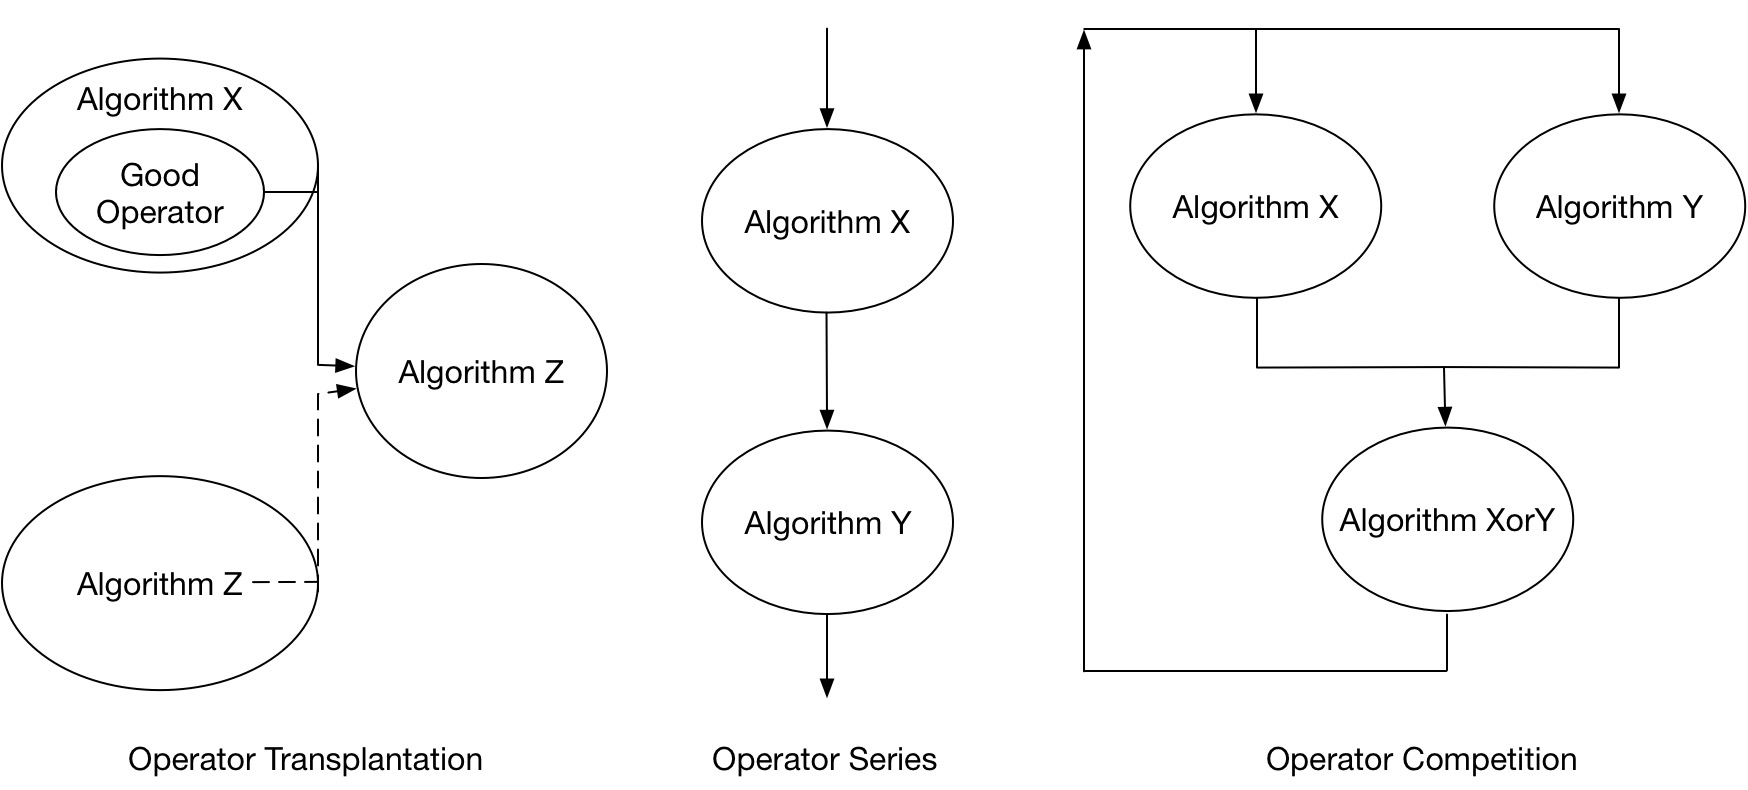
\includegraphics[height=4cm]{img/hybrid_immune.jpg}
\end{center}
\end{frame}

\begin{frame}{Hybrid Immune Algorithm}
\begin{itemize}\large{
\item{Immune Genetic Algorithm}
\item{Immune Particle Swarm Optimization}
\item{Synergetic Evolutionary Immune Algorithm}
\item{Immune Ant colony algorithm}
\item{
Quantum Immune Algorithm\\
Chaotic Immune Algorithm\\
Fuzzy Immune System\\
Immune Neural Network Algorithm\\
......
}}
\end{itemize}
\small
{\noindent

}
\end{frame}

\begin{frame}{Immune Ant Colony Algorithm}{Ant Colony Algorithm}
 \huge \textbf{Ant Colony Algorithm}\\~\\
 \large
 {
Ants leave a \textcolor{red}{pheromone} in the path that it travels when foraging, and can feel the intensity of it during the movement and tend to move in the direction of \textcolor{red}{high concentration}, so the  group behavior will show \textcolor{red}{positive feedback} with pheromone information.
 }\\
\end{frame}

\begin{frame}{Immune Ant Colony Algorithm}{Problems and Solving}
\begin{table}
\begin{tabular}{p{11em}|p{19em}}
\toprule
\textbf{Ant Colony Weakness} & \textbf{Immune Algorithms Advantages}\\
\midrule \small
\footnotesize{Lack of information at first, convergence slows} & \footnotesize{ \textcolor{red}{Clone mutation mechanism}, use affinity describe the matching between antibody and antigen, fast global search capabilities}\\
\footnotesize{Easy to fall into local extreme point and premature convergence occurs} & \footnotesize{ \textcolor{red}{Concentration inhibition mechanism}, influencing road path selection probability to maintain the ant colony diversity} \\
\bottomrule
\end{tabular}
\end{table}
\end{frame}

\begin{frame}{Immune Ant Colony Algorithm}{TSP}
 \large \textbf{Traveling Salesman Problem}\\~\\
 {TSP is a \textcolor{red}{shortest path problem}. For n cities, choose any cities as the starting point and traverse all the cities back to the starting point. When the sum of the paths is the \textcolor{red}{shortest}, the path is optimal.}
 \begin{equation} \small{
 T_{d}=\sum_{i=1}^{n-1}d\left (v_{i},v_{i+1}\right )+d\left (v_{1},v_{n} \right)}
 \end{equation}
\end{frame}

\begin{frame}{Immune Ant Colony Algorithm}{Term Definition}
\large \textbf{Term Definition}\\~\\
\begin{itemize}
\item \textbf{Antigen}
\item \textbf{Antibody}
\begin{equation}\small{
  D=\left \{\left \langle s,T_d\right \rangle | s \in P , T_d \in N \right \}}
\end{equation}
\item \textbf{Affinity}
\small{
\begin{equation}
  f_{dist}\left(A_{b},A_{g} \right) = 1 /\left(A_{b}.dist - A_{g}.dist\right)
\end{equation}
\begin{equation}
  T = \left(\sum_{i=1}^{n} \sum_{j=1}^{n}d\left(i,j\right)\right)/\left(2n\right)
\end{equation}
\begin{equation}
  f_{dist}\left(A_{b},A_{g} \right) = 1 /\left(A_{b}.dist - T\right)
\end{equation}}
\end{itemize}
\end{frame}

\begin{frame}{Immune Ant Colony Algorithm}{Term Definition}
\large \textbf{Term Definition}\\~\\
\begin{itemize}
\item \textbf{Memory Cells}
\begin{equation} \small{
  M=\left \{ x |f_{dist} \left(A_{b},A_{g}\right)\geqslant \theta,x \in D \right \}}
\end{equation} \small{
\item \textbf{Path Transition Probability}}
\begin{equation}
p{_{ij}}^{k} =
\begin{cases}
\frac{[\tau_{ij}(t)]^\alpha \cdot [\eta_{ij}]^\beta} { \sum\limits_{s \subset allowed_{k}} [\tau_{is}(t)]^\alpha \cdot [\eta_{is}(t)]^\beta} & j \in allowed_k \\
0 & else
\end{cases}
\end{equation}
\end{itemize}
\end{frame}

\begin{frame}{Immune Ant Colony Algorithm}{Algorithms Step}
\large \textbf{Step1 Calculate a feasible solution using immune algorithm}\\~\\
\begin{itemize}
\item{Enter question and determine the antibody encoding}
\item{Calculate antibody affinity $f_{dist}$, Memory cell $M(f_{dist}\geqslant\theta)$}
\item{Antibody clone variation \qquad $A_{bj}\rightarrow C_j \rightarrow C_j^*$}
\begin{equation}\small{
i=INT[num \times \beta \div con]}
\end{equation}
\begin{equation}\small{
con_i=\frac{M_{bi}}{M_{b}} }
\end{equation}
\item{Update group \qquad \small{$f_{dist}(A_{bj}^*,A_{gj}) > f_{dist}(A_{bj},A_{gj}) ?$}} 
\item{Terminal condition}
\end{itemize}
\end{frame}

\begin{frame}{Immune Ant Colony Algorithm}{Algorithms Step}
\large \textbf{Step2 Initialize the pheromone based on feasible solution}\\~\\
\begin{equation}
\tau_{ij}(0)=
\begin{cases}
\tau_C +\tau_G & e_{ij} \in L^* \\
\tau_C & else
\end{cases}
\end{equation}
\begin{equation}
\tau_G = \frac{Q}{L^*}
\end{equation}
\centering \small{
{$\tau$:pheromone amount}\\ {$Q$: a cycle pheromone amount}\\ {$L^*$:optimal path length}
}
\end{frame}

\begin{frame}{Immune Ant Colony Algorithm}{Algorithms Step}
\large \textbf{Step3 Construct probability formula using immune inhibition operators}\\~\\
\centering \small { \textcolor{red}{Path Concentration $C_{ij}$:} the amount of ants that choose path $e_{ij}$}
\begin{equation}\small{
C_{ij}(t) = \frac{1}{M} \sum\limits_{k=1}^{M}iif \left(e_{ij} \in Tour^k(t),1,0\right)}
\end{equation}
\begin{equation}\small{
C_{ij}^k(t) = \frac{1}{M} \sum\limits_{k=1}^{k-1}iif \left(e_{ij} \in Tour^k(t),1,0\right)}
\end{equation}
\end{frame}

\begin{frame}{Immune Ant Colony Algorithm}{Algorithms Step}
\large \textbf{Step3 Construct probability formula using immune inhibition operators}\\~\\
\centering \small {Update pheromone amount $\tau_{ij}$ considering path concentration $c_{ij}$}
\begin{equation}
\tau_{ij}^k(t)=
\begin{cases}
\tau_{ij} \cdot \left(\lambda \cdot c_{ij}^k(t)\right) & if \quad c_{ij}^k(t) > c_0 \\
\tau_{ij} & else
\end{cases}
\end{equation}
\begin{equation}
p{_{ij}}^{k} =
\begin{cases}
\frac{[\tau_{ij}^k(t)]^\alpha \cdot [\eta_{ij}]^\beta} { \sum\limits_{\mu \subset N^k_l(t)} [\tau_{i\mu}^k(t)]^\alpha \cdot [\eta_{i\mu}(t)]^\beta} & if j \in N^k_i(t) \\
0 & else
\end{cases}
\end{equation}
\end{frame}

\begin{frame}{Immune Ant Colony Algorithm}{Algorithms Step}
\large \textbf{Step4 Update pheromones}\\~\\
\begin{equation} \small{
\tau_{ij}(t+n) = (1-\omega)\cdot\tau_{ij}(t)+\omega\cdot C}
\end{equation} \\~\\
\centering \small {Update the pheromone of shortest path and longest path}
\begin{equation}\small{
\tau_{ij}(t+n) = (1-\rho)\cdot\tau_{ij}(t)+\rho\cdot \Delta{\tau_{ij}}'(t)}
\end{equation}
\begin{equation} \small{
\Delta{\tau_{ij}}'(t) = 
\begin{cases}
\frac{Q}{L_{best}} & e_{ij} \in L_{best} \\
-\frac{Q}{L_{worst}} & e_{ij} \in L_{worst} \\
0 & else
\end{cases}}
\end{equation}
\end{frame}

\begin{frame}{Summary}
\large \textbf{Two tyeps of Hybrid Immune Algorithms} \\~\\
\begin{itemize}
\item{Introduce the immune concept and mechanism into other algorithms, overcome local extreme points and improve convergence accuracy}
\item{Introduce other algorithms into immune algorithm, increase the convergence speed of algorithm}
\end{itemize}
\end{frame}

\begin{frame}
\centering \Huge \textbf{Thank You!}
\end{frame}
